\chapter{Implementación}
\label{cap:implementacion}

\chapterquote{Puede que tengas grandes ideas en la cabeza, pero lo que importa es la acción. Una idea, si no se lleva a cabo, no producirá ninguna manifestación, ni resultados ni recompensas}{Miguel Ruiz}


En este capítulo hacemos una descripción detallada sobre la arquitectura en la que está basada nuestro asistente. Hablaremos también sobre la implementación de las distintas funcionalidades (ver sección XXXX) que se ha llevado a cabo tanto en la parte Back End como Front End.


\section{Arquitectura}

La estructura de nuestro proyecto está soportado sobre un entorno Flask, teniendo el nivel de directorios que se muestra en la Figura \ref{fig:projectStructure}.

	 \begin{figure}[h!]
	\centering
	
	
	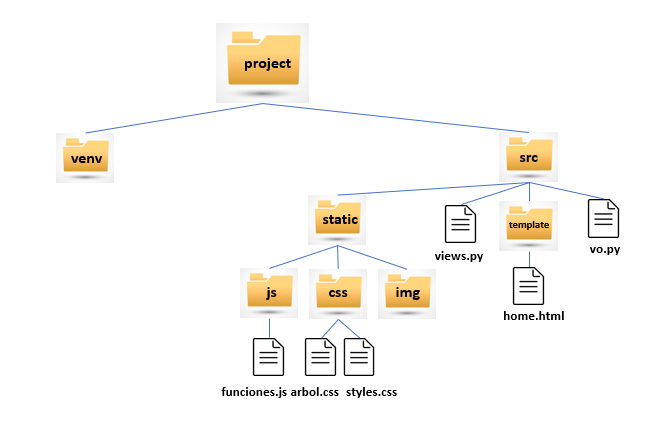
\includegraphics[scale=1.2]{Imagenes/Figuras/Project-Structure}
	
	
	\caption{Estructura del proyecto en Flask}
	\label{fig:projectStructure}
\end{figure}

A continuación, se explican la función de cada uno de los ficheros que componen la aplicación web.

\subsection{Ficheros del entorno}

Los ficheros principales son:
\begin{itemize}
	\item \textbf{views.py}: es el encargado de la lógica de todos los endpoints de la aplicación, así como el renderizado de la plantilla. Cada uno de esos endpoints tendrá una funcionalidad distinta, los cuales serán llamados por una función de funciones.js 
	\item \textbf{vo.py}: se encarga de la organización de clases.
	\item \textbf{home.html}: en este archivo creamos la estructura de nuestro asistente y la organización que mostrará el contenido.
	\item \textbf{funciones.js}: la misión de este fichero es comunicar la aplicación web con los elementos del DOM de la misma, haciendo posible la modificación del HTML dinámicamente. Las modificaciones que efectuamos en este archivo es añadir nuevas etiquetas, modificando o eliminando otras, cambiar sus atributos, añadiendo clases, cambiar el contenido de texto, etc. También es el encargado de la comunicación con la vista (views.py) para la petición y respuesta de servicios web.
	\item \textbf{arbol.css}: archivo encargado de generar los estilos para que nuestro árbol de dependencias tenga la apariencia de un árbol genealógico.
	\item \textbf{style.css}: fichero encargado de dar estilos a todo lo que concierne nuestra aplicación web excepto el árbol de dependencias (fuentes, disposición, tamaños, colores, etc.)   
\end{itemize}

\subsection{Servicios web externos}\label{sec:serviciosWebExternos}
Para hacer uso de las principales funcionalidades descritas en la sección XXX, contamos con una arquitectura de servicios web REST basada en endpoints (URLs), intercambiando mensajes entre cliente y servidor (Figura \ref{fig:apiRest}). 

\begin{figure}[h!]
	\centering
	
	
	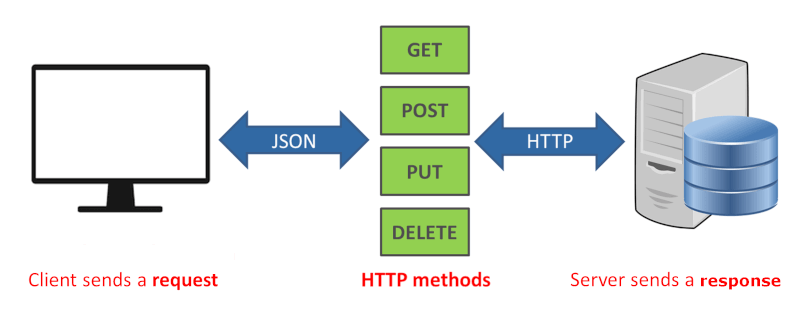
\includegraphics[scale=0.4]{Imagenes/Figuras/rest_api}
	
	
	\caption{Servicio REST cliente/servidor}
	\label{fig:apiRest}
\end{figure}

Un servicio web REST es una interfaz para conectar varios servicios web basados en el protocolo HTTP que define una gran cantidad de métodos, de los cuales describimos los cuatro más básicos:
\begin{itemize}
	\item \textbf{GET}: se utiliza para acceder a los distintos recursos. Si requiere del envío de un parámetro al servidor (URI param), éste se pasa como un elemento en la URI (del inglés, \textit{Uniform Resource Identifier}). 
	
	\item \textbf{POST}: se usa para realizar acciones de creación de nuevos recursos. Si se requiere el envío de información al servidor, esta se pasa dentro del cuerpo de la petición HTTP (body param).
	
	\item \textbf{PUT}: se utiliza para la modificación de los recursos existentes. Puede enviar parámetros tanto en la URI como en el cuerpo de la petición HTTP.
	
	\item \textbf{DELETE}: se utiliza para la eliminar los recursos existentes, siendo la operación análoga al POST. El parámetro será informado a través de la URI.
\end{itemize}

Estas métodos pueden ser usados en distintas situaciones devolviendo los datos en distintos formatos como XML y JSON.
En nuestro caso, hemos usado el formato JSON.

Nuestra arquitectura REST tiene el aspecto como muestra la Figura \ref{fig:ArquitecturaAsistenteR}, que a continuación describimos.
\begin{figure}[h!]
	\centering
	
	
	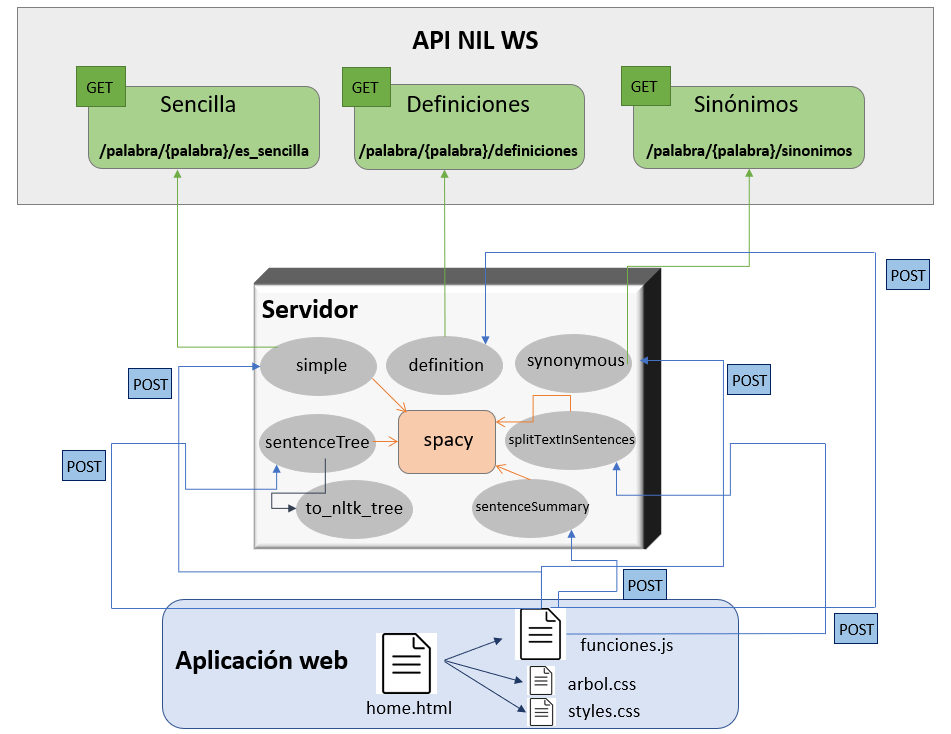
\includegraphics[scale=0.9]{Imagenes/Figuras/ArquitecturaAsistenteR}
	
	
	\caption{Diagrama de la arquitectura REST del asistente web}
	\label{fig:ArquitecturaAsistenteR}
\end{figure}

  Hacemos uso de los siguientes servicios REST que nos ofrece la API del grupo NIL\footnote{Para más información acceder a \href{https://holstein.fdi.ucm.es/nil-ws-api/}{https://holstein.fdi.ucm.es/nil-ws-api/}} (descrita en el capítulo X sección XXX):


	


\begin{itemize}
	\item \textbf{Servicio para comprobar si una palabra es compleja}.
	\begin{lstlisting}[backgroundcolor = \color{pink},
	xleftmargin = 1cm,
	framexleftmargin = 1em,frame=tlbr,framesep=4pt,framerule=1pt]
	GET https://holstein.fdi.ucm.es/nil-ws-api/palabra/
	{palabra}/es\_sencilla
	
	
\end{lstlisting}
	
	Este recurso devuelve un objeto en formato JSON que contiene el campo ``palabraSencilla'' de tipo booleano que en el caso que sea False la palabra introducida a través de la URI es compleja (ver Figura \ref{fig:apiSencilla}).
		 \begin{figure}[h!]
		\centering
		
		
		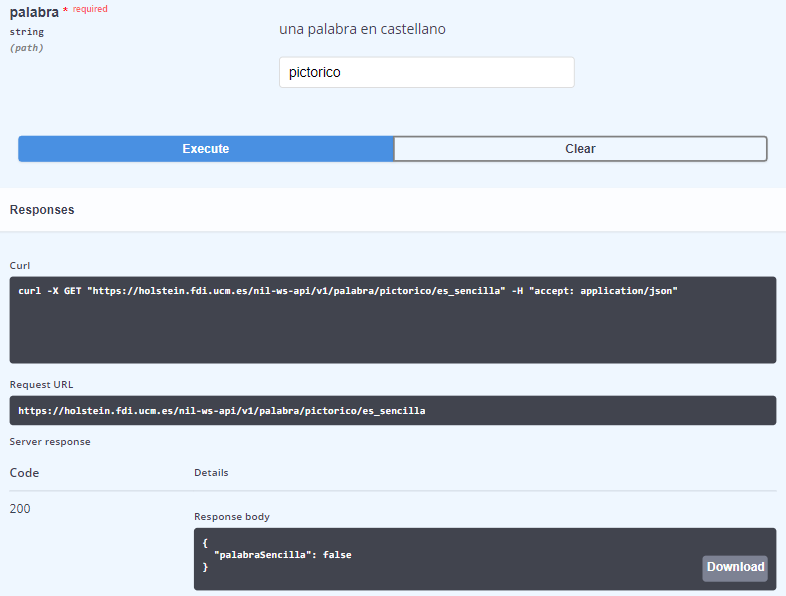
\includegraphics[scale=1]{Imagenes/Figuras/APISencilla}
		
		
		\caption{Petición para comprobar si una palabra es compleja}
		\label{fig:apiSencilla}
	\end{figure}
	\item \textbf{Servicio para obtener definiciones de una palabra}.
\newline

	\begin{lstlisting}[backgroundcolor = \color{pink},
	xleftmargin = 1cm,
	framexleftmargin = 1em,frame=tlbr,framesep=4pt,framerule=1pt]
	GET https://holstein.fdi.ucm.es/nil-ws-api/palabra/
	{palabra}/definiciones

	
	
\end{lstlisting}




En este caso, el servicio devuelve un objeto JSON que contiene el campo ``definiciones'' de tipo arrayList en el que en cada posición hay otro objeto, ``definicion'', cuyo valor es de tipo string con la acepción correspondiente (ver Figura \ref{fig:apiDefinicion}).
\begin{figure}[h!]
	\centering
	
	
	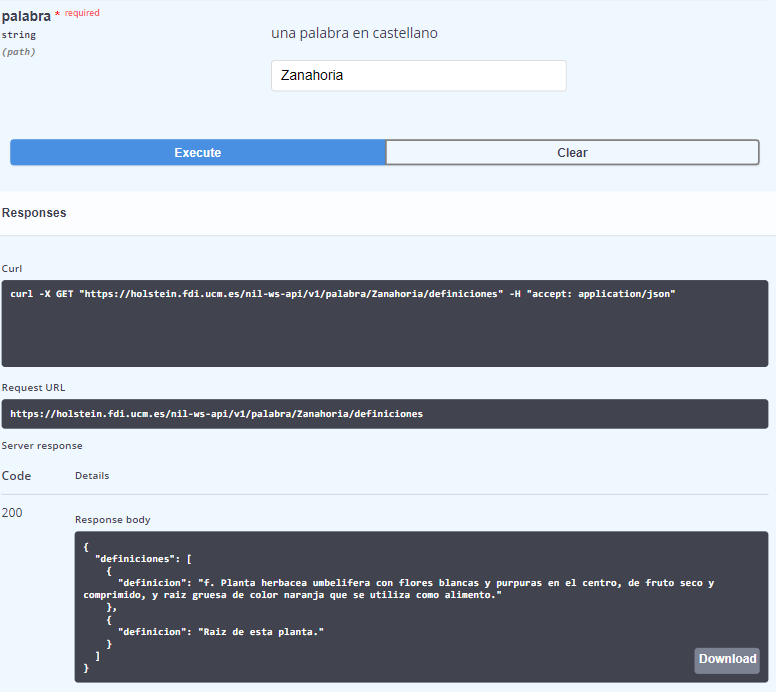
\includegraphics[scale=1]{Imagenes/Figuras/ApiDefinicion}
	
	
	\caption{Petición que devuelve una lista de definiciones}
	\label{fig:apiDefinicion}
\end{figure}
	\item \textbf{Servicio para obtener sinónimos de una palabra}.
	\begin{lstlisting}[backgroundcolor = \color{pink},
	xleftmargin = 1cm,
	framexleftmargin = 1em,frame=tlbr,framesep=4pt,framerule=1pt]
	GET https://holstein.fdi.ucm.es/nil-ws-api/palabra/
	{palabra}/sinonimos	
	
	
	
	
\end{lstlisting}



El servicio devuelve un objeto JSON que contiene el campo ``sinonimos'' de tipo arrayList en el que en cada posición hay otro objeto, ``sinonimo'', cuyo valor es de tipo string con la acepción correspondiente (ver Figura \ref{fig:apiSinonimo}).
\begin{figure}[h!]
	\centering
	
	
	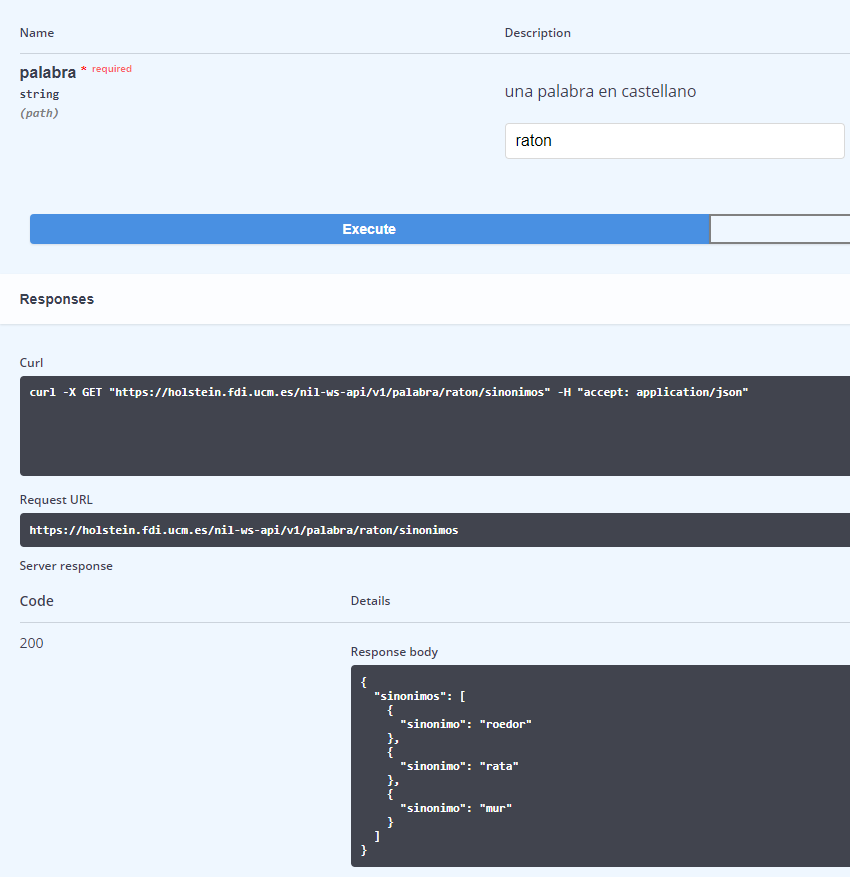
\includegraphics[scale=1]{Imagenes/Figuras/APISinonimos}
	
	
	\caption{Petición que devuelve una lista de sinónimos}
	\label{fig:apiSinonimo}
\end{figure}
\end{itemize}

Cabe destacar que esta API no hace uso de las reglas de acentuación, de manera que debemos de insertar las palabras sin tildes (obsérvese la Figura \ref{fig:apiSinonimo}).

\subsection{Librería Spacy}

\subsection{Implementaciones del servidor}

\subsection{Implementaciones de la aplicación web}

En esta sección se explica en detalle como han sido desarrolladas las funcionalidades (capítulo \ref{cap:asistenteWeb} \ref{sec:}) de la aplicación web, cuya finalidad es proporcionar al usuario una interfaz sencilla, donde puedan introducir un texto, hacer una serie de transformaciones para obtener el mismo simplificado a Lectura Fácil.


Para que el contenido de la aplicación web sea dinámico se ha desarrolla con JavaScript, cambiando según la acción del usuario. Estás acciones son:

\begin{itemize}
	\item Botón (\textbf{Resumen}): se realiza una llamada Fetch al endpoint ``/summary'' con el texto completo previamente introducido. La respuesta recibida será un objeto JSON, el cuál contiene el resumen del texto. Posteriormente se hará otra llamada Fetch al endpoint ``/sentences'', que devuelve el texto en frases. Estás frases se incrustan en el código HTML, escribiéndolas a modo de lista (una debajo de otra).    
 
	\item Botón (\textbf{Texto completo}): a diferencia de botón anterior este hace una llamada únicamente al endpoint ``/sentences'', devolviendo el texto completo en frases.

	\item Creación del árbol de dependencias: se realiza una llamada Fetch al endpoint ``/sentences/tree'', devolviendo así un objeto JSON con la estructura del árbol. Para su construcción de este, hemos usado un algoritmo de búsqueda en profundidad (BFS), recorriendo todos los nodos (en nuestro caso palabras de la frase). El funcionamiento de este algoritmo consiste en ir expandiendo cada uno de sus nodos desde la raíz hacia el nodo hoja (no tiene más hijos) de manera recurrente (Figura \ref{fig:diagramaBFS}).
	\begin{figure}[h!]
		\centering
		
		
		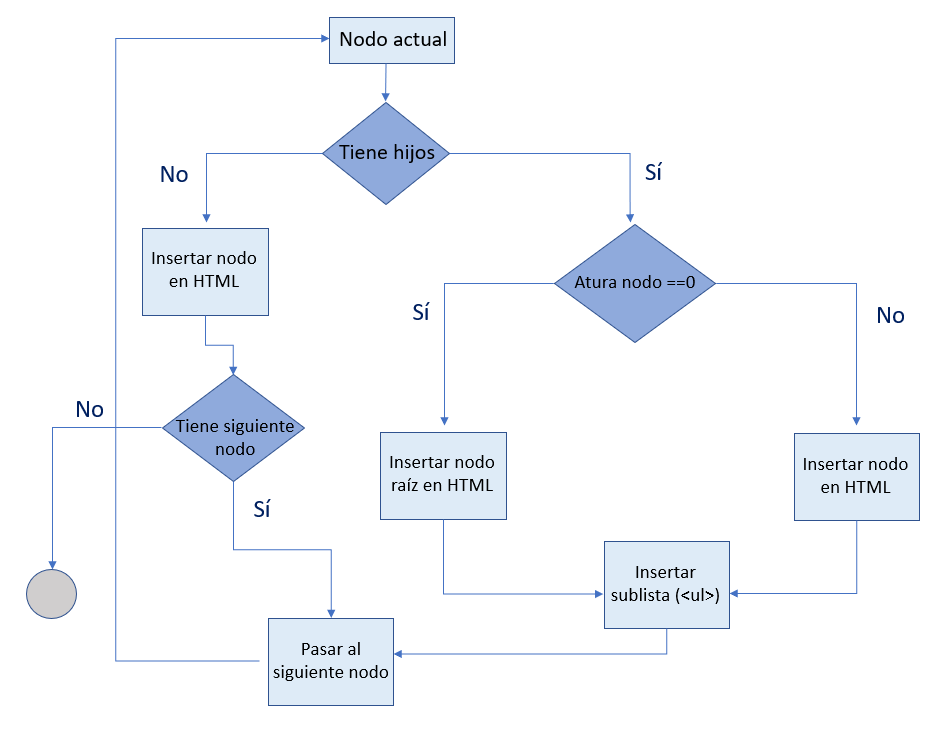
\includegraphics[scale=1]{Imagenes/Figuras/diagramaBFS}
		
		
		\caption{Petición que devuelve una lista de sinónimos}
		\label{fig:diagramaBFS}
	\end{figure}
	
		Por ejemplo, supongamos que queramos adaptar la frase ``También se instalarán 2.500 cabinas para que los electores puedan seleccionar su papeleta en secreto si así lo desean.'', el objeto JSON tendría el aspecto de la Figura \ref{fig:objetoJSON}. 
	Cada nodo contiene los siguientes datos:
		\begin{itemize}
		\item \textbf{children}: array de nodos hijos.
		\item \textbf{height}: nivel del nodo con respecto a la raíz (en nuestro ejemplo ``instalarán'' sería nuestra raíz, que tiene una altura 0).
		\item \textbf{id}: identificador único de cada nodo.
		\item \textbf{text}: palabra propia del nodo.
	\end{itemize}
En la Figura \ref{fig:arbolDependencias} observamos el árbol con el que podremos interactuar durante la adaptación.
	\item Palabras complejas.
	\item 
\end{itemiz